\section*{Форматы входных и выходных файлов}

Файлы для списков грузовиков хранятся в формате CSV (Comma Separated Values). 
В каждом файле присутствует заголовочная строка, 
показывающая какие данные хранятся в каждом столбце. 
Данные в столбцах разделяются запятыми.
Для загружаемых и сохраняемых списков формат один и тот же.

Для грузовиков определены следующие столбцы:
\begin{itemize}
    \item id -- идентификационный номер грузовика (int);
    \item brand -- марка грузовика (std::string);
    \item capacity -- грузоподъёмность грузовика в тоннах (float);
    \item transportation\_distance -- максимальная дальность перевозки (int).
\end{itemize}

Пример файла пердставлен на рис. \ref{file_example}

\begin{figure}[hpt!]
    \centering
    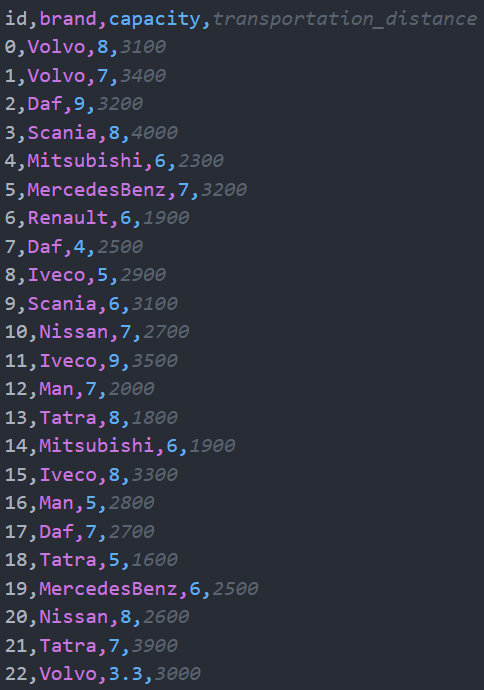
\includegraphics[width=0.5\linewidth]{photo/file_example}
    \caption{Пример таблицы грузовиков}
    \label{file_example}
\end{figure}